\chaptertitle{第三章\quad 计数原理}

前两章建立了语言和推理工具，本章进入组合数学的核心——计数。"一共有多少种可能"是许多组合问题的最终目标。我们从两个最基础的原理开始，它们听起来简单，但灵活运用起来可以解决大量问题。

\sectiontitle{3.1\quad 加法原理}

先看三个问题：
\begin{enumerate}
\item 小红的衣柜里有$3$条裙子、$2$条裤子，她想穿一条裙子或一条裤子出门，有多少种选择？
\item 从北京到上海，可以坐高铁（$5$趟）、飞机（$3$班）或大巴（$2$班），有多少种方式？
\item 书架上有$4$本数学书和$3$本语文书，想拿一本数学书或一本语文书，有多少种拿法？
\end{enumerate}

\begin{example}
分别计算以上三个问题。
\end{example}
\begin{solution}
(1) $3+2=5$种。\qquad (2) $5+3+2=10$种。\qquad (3) $4+3=7$种。
\end{solution}

\textbf{加法原理（分类计数）}：完成一件事有$n$类不同的方式，第$i$类有$m_i$种方法，且各类方法之间互不重叠（任何两种方法都不同），那么完成这件事总共有
\[
N = m_1 + m_2 + \cdots + m_n
\]
种不同的方法。

加法原理的本质是"分类相加"——各选各的，互不干扰，加起来就是总数。

\begin{example}
从$1$到$10$中任取一个数，取到质数或偶数的取法有多少种？
\end{example}
\begin{solution}
质数：$\{2,3,5,7\}$共$4$个；偶数：$\{2,4,6,8,10\}$共$5$个。\\
注意$2$既是质数又是偶数，两类有重叠。\\
所以不能用简单的$4+5$。正确做法：质数或偶数的数量$=4+5-1=8$（去掉重复的$2$）。\\
这实际上是下一章要学的容斥原理的雏形。
\end{solution}

\sectiontitle{3.2\quad 乘法原理}

再来看三个问题：
\begin{enumerate}
\item 小红有$3$件上衣和$4$条裤子，想穿一件上衣搭配一条裤子出门，有多少种搭配？
\item 从$A$地到$B$地有$3$条路，从$B$地到$C$地有$2$条路，从$A$到$C$经过$B$有多少种走法？
\item 一个两位数的十位可以从$1$到$9$中选，个位可以从$0$到$9$中选，能组成多少个不同的两位数？
\end{enumerate}

\begin{example}
分别计算以上三个问题。
\end{example}
\begin{solution}
(1) 选上衣有$3$种，每条上衣配$4$条裤子：$3\times4=12$种。\\
(2) $A\to B$有$3$种走法，每种接$B\to C$的$2$种走法：$3\times2=6$种。\\
(3) 十位$9$种选法，个位$10$种选法：$9\times10=90$种。
\end{solution}

\textbf{乘法原理（分步计数）}：完成一件事需要$n$个步骤，第$i$步有$m_i$种方法，且各步之间相互独立（前一步的每种选择与后一步的每种选择都能搭配），那么完成这件事总共有
\[
N = m_1 \times m_2 \times \cdots \times m_n
\]
种不同的方法。

乘法原理的本质是"分步相乘"——一步选完再接一步，所有可能性乘起来。

\begin{center}
\begin{tikzpicture}[scale=0.6]
% 树形图示意
\node at (0,2) {上衣1};
\node at (0,0) {上衣2};
\node at (0,-2) {上衣3};
\node at (3,2.5) {裤A};
\node at (3,1.5) {裤B};
\node at (3,0.5) {裤C};
\node at (3,-0.5) {裤D};
\node at (3,-1.5) {裤A};
\node at (3,-2.5) {裤B};
\node at (3,-3.5) {裤C};
\node at (3,-4.5) {裤D};
\draw[->] (0.3,2) -- (2.7,2.3);
\draw[->] (0.3,2) -- (2.7,1.3);
\draw[->] (0.3,2) -- (2.7,0.3);
\draw[->] (0.3,2) -- (2.7,-0.7);
\draw[->] (0.3,0) -- (2.7,-1.7);
\draw[->] (0.3,0) -- (2.7,-2.7);
\draw[->] (0.3,-2) -- (2.7,-3.7);
\draw[->] (0.3,-2) -- (2.7,-4.7);
\node at (1.5,-6) {树形图：$3$件上衣$\times4$条裤子$=12$种搭配};
\end{tikzpicture}
\end{center}

\begin{exercise}
\item 食堂有$4$种荤菜和$3$种素菜，选一荤一素有多少种搭配？
\item 用$1,2,3,4$能组成多少个无重复数字的三位数？
\item 从$A$到$B$有$2$条路，$B$到$C$有$3$条路，$C$到$D$有$4$条路，$A$到$D$经过$B$和$C$有多少种走法？
\end{exercise}

\sectiontitle{3.3\quad 加法与乘法的区分与综合}

实际问题的复杂之处在于：加法原理和乘法原理很少单独出现——它们需要组合使用。

判断用加法还是乘法的关键：
\begin{itemize}
\item \textbf{分类用加法}："或"关系——做这件事有几种不同的类别，每一类都能独立完成这件事。
\item \textbf{分步用乘法}："且"关系——做这件事需要依次完成几个步骤，缺一不可。
\end{itemize}

\begin{example}
用$1,2,3,4,5$五个数字能组成多少个无重复数字的偶数？
\end{example}
\begin{solution}
分步：先定个位（偶数有$2,4$两种），再定十位（剩下$4$个数字选$1$），再定百位（剩下$3$个选$1$）：
$2\times4\times3=24$个。
\end{solution}

\begin{example}
小明要从家到学校，可以步行（$15$分钟）、骑自行车（$8$分钟）或坐公交（$10$分钟）。放学后他要先去图书馆（从学校到图书馆有$3$种走法），再回家（从图书馆到家有$2$种走法）。问：小明从家到学校，以及放学后从学校经图书馆回家的路线各有多少种？
\end{example}
\begin{solution}
从家到学校：$3$种方式（加法原理，三类选一）。\\
放学后$学校\to图书馆\to家$：$3\times2=6$种（乘法原理，分两步）。
\end{solution}

\begin{example}
用$0,1,2,3$能组成多少个无重复数字的三位数？
\end{example}
\begin{solution}
百位不能是$0$，所以百位有$3$种（$1,2,3$）。\\
十位可从剩下$3$个中选（包括$0$）：$3$种。\\
个位从剩下$2$个中选：$2$种。\\
总数：$3\times3\times2=18$个。
\end{solution}

\begin{exercise}
\item 用$0,2,4,6,8$能组成多少个无重复数字的三位偶数？
\item 某餐厅有$3$种主食和$5$种菜品。一份套餐可选一种主食配一种菜品，或单点一种菜品。一共有多少种不同的点餐方式？
\end{exercise}

\sectiontitle{3.4\quad 图形计数}

图形计数是加法原理和乘法原理的经典应用——数一数图形中有多少条线段、多少个三角形、多少个长方形。

\begin{example}
下图中有多少条线段？
\[
A\;-\;B\;-\;C\;-\;D\;-\;E
\]
\end{example}
\begin{solution}
方法一（分类枚举）：\\
长度为$1$的线段：$AB,BC,CD,DE$（$4$条）。\\
长度为$2$的：$AC,BD,CE$（$3$条）。\\
长度为$3$的：$AD,BE$（$2$条）。\\
长度为$4$的：$AE$（$1$条）。\\
总计$4+3+2+1=10$条。

方法二（选端点）：每条线段由两个端点确定。$5$个点中选$2$个：根据组合公式（后两章会学）$\dfrac{5\times4}{2}=10$条。
\end{solution}

\begin{example}
下图中有多少个三角形？
\[
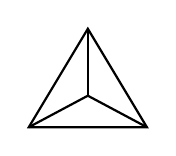
\begin{tikzpicture}[scale=0.5]
\draw[thick] (0,0) -- (3,0) -- (1.5,2.5) -- cycle;
\draw[thick] (0,0) -- (1.5,0.8);
\draw[thick] (1.5,0.8) -- (3,0);
\draw[thick] (1.5,0.8) -- (1.5,2.5);
\end{tikzpicture}
\]
\end{example}
\begin{solution}
按大小分类：\\
小三角形（被分割出的最小块）：$4$个。\\
中等三角形（由$2$个小块组成）：$3$个。\\
大三角形（由$4$个小块组成）：$1$个。\\
总计$4+3+1=8$个。
\end{solution}

\begin{example}
$3\times4$的网格（$4$行$3$列小方格）中有多少个长方形（含正方形）？
\end{example}
\begin{solution}
一个长方形由两条竖线和两条横线围成。\\
$4$行有$5$条横线，选$2$条：$\dfrac{5\times4}{2}=10$种。\\
$3$列有$4$条竖线，选$2$条：$\dfrac{4\times3}{2}=6$种。\\
总数：$10\times6=60$个长方形。
\end{solution}

\begin{exercise}
\item 数一数下图中有多少条线段：$A\;-\;B\;-\;C\;-\;D$。
\item 从$n$个点中任选$2$个可以确定一条线段，$n$个点最多有多少条线段？
\item $2\times2$的网格（$2$行$2$列小方格）中有多少个长方形？
\end{exercise}

\sectiontitle{3.5\quad 枚举策略}

当问题实在找不到简便公式时，最可靠的方法就是枚举——把所有可能一一列出来。枚举的关键是\textbf{不重不漏}。

常用枚举策略：
\begin{enumerate}
\item \textbf{有序枚举}：按一定顺序（从小到大、从少到多）列举，避免遗漏。
\item \textbf{分类枚举}：把问题分成几类，对每类分别枚举。
\item \textbf{树形图}：用树状结构展示枚举过程。
\end{enumerate}

\begin{example}
用$1$元、$2$元、$5$元纸币各一张，可以组成多少种不同的币值？
\end{example}
\begin{solution}
按取几张分类枚举：\\
取$1$张：$1$元、$2$元、$5$元——$3$种。\\
取$2$张：$1+2=3$元、$1+5=6$元、$2+5=7$元——$3$种。\\
取$3$张：$1+2+5=8$元——$1$种。\\
总计$3+3+1=7$种。
\end{solution}

\begin{example}
甲、乙、丙三人进行乒乓球比赛，每两人赛一场，所有可能的胜负结果有多少种？
\end{example}
\begin{solution}
共有$3$场比赛：甲vs乙、甲vs丙、乙vs丙。\\
每场比赛有$2$种结果（甲胜或乙胜等）。\\
由乘法原理：$2\times2\times2=8$种胜负结果。
\end{solution}

枚举法看似"笨"，但它是最不容易出错的方法，也是理解更高级计数技巧的基础。当你对一个问题没有头绪时，先尝试枚举几个简单情形，往往能发现规律。

\begin{exercise}
\item 用树形图列出$1$枚硬币抛$3$次的所有可能结果（正面/反面）。
\item 从$1,2,3$中选若干个数（至少一个），可以组成多少种不同的和？
\end{exercise}

\sectiontitle{本章小结}

本章学习组合数学最基础的两个计数工具：加法原理（分类相加）和乘法原理（分步相乘）。它们的核心区别在于"或"与"且"的逻辑关系。图形计数是这两个原理的综合应用。当公式难以直接使用时，枚举法是最可靠的保障。后续各章的排列、组合、隔板法等方法，本质上都是从加乘原理出发推导出的高效计数工具。

\sectiontitle{课后练习}

\subsection*{A组\quad 基础巩固}

\begin{exercise}
\item 小明有$5$种不同的铅笔和$3$种不同的橡皮，买一支铅笔加一块橡皮有多少种搭配？
\item 从$A$到$B$有$4$条路，$B$到$C$有$3$条路，$A$直接到$C$有$2$条路。从$A$到$C$共有多少种走法？
\item 用$1,2,3,4$能组成多少个无重复数字的四位数？
\item 数一数$A\;-\;B\;-\;C\;-\;D\;-\;E\;-\;F$中有多少条线段。
\item 书架上有$3$本不同的数学书和$4$本不同的语文书。想拿两本书（一本数学一本语文）有多少种拿法？
\end{exercise}

\subsection*{B组\quad 挑战提升}

\begin{exercise}
\item 用$0,1,2,3,4$能组成多少个无重复数字且大于$200$的三位数？
\item $4$对夫妇站成一排拍照，要求每对夫妇都相邻，有多少种站法？（提示：分两步——先排$4$对夫妇，再考虑每对内部的左右顺序。）
\item 有$1$元、$2$元、$5$元、$10$元纸币各一张，可以组成多少种不同的币值？
\item $m\times n$的网格（$m$行$n$列小方格）中有多少个长方形？
\end{exercise}

\vfill
\noindent\rule{\textwidth}{0.4pt}
本章练习答案请参见书末附录。
